\section{Method}
\label{sec:method}
\begingroup
\setlength{\abovedisplayskip}{5pt plus 2pt minus 2pt}
\setlength{\belowdisplayskip}{5pt plus 2pt minus 2pt}
\setlength{\abovedisplayshortskip}{3pt plus 2pt minus 1pt}
\setlength{\belowdisplayshortskip}{4pt plus 2pt minus 1pt}
\setlength{\jot}{2pt}

\subsection{Framework Overview}

\textsc{FinOPD} separates what evolves from when it may evolve. Alpha-Factor Evolution first compiles and freezes a versioned library of executable expressions. In each OPD round, the current student produces trajectories from point-in-time information. Only after an outcome horizon closes may the frozen teacher inspect an estimated hindsight summary, the student and router update, and a finalized episode enter long-term memory. This schedule pairs a parametric policy with auditable factors and local experience.
% 中文翻译：FinOPD 同时区分“哪些知识发生进化”和“何时允许进化”。Alpha-Factor Evolution 首先构建并冻结带版本的可执行表达式库。每一轮 OPD 中，当前学生只利用时点可得信息生成轨迹；只有结果窗口闭合后，冻结教师才能读取估计的事后摘要，学生与路由器才允许更新，最终情节也才允许进入长期记忆。该时间表把参数策略轨道与保存可审计因子和局部经验的非参数轨道结合起来。

Figure~\ref{fig:architecture} instantiates this chronology. Point-in-time geometry and routed factors enter a five-agent chain whose decision-local Gated Shared Memory preserves provenance, confidence, and disagreement before being reset. Cross-time episodic memory is updated separately from matured records.
% 中文翻译：图 2 展示了这一时间顺序。时点可得的图形几何与路由因子进入五智能体链；决策局部的 Gated Shared Memory 保留证据来源、置信度和分歧，并在决策后重置。跨时间情节记忆则通过独立流程写入已经成熟的记录。

\subsection{Financial Multi-Agent Decision Backbone}

\paragraph{Visual-geometric representation.}
\label{sec:vge}
The Visual-Geometric Encoder adapts Qwen3.5-9B~\cite{qwen35_2026} with rank-16 LoRA on its upper vision and cross-attention layers. It maps each point-in-time chart to validated \texttt{ChartGeometry} fields covering trend lines, support and resistance, formations, volume cues, and regime descriptors. This structured interface targets the spatial and instruction-following failures documented by FinChart-Bench~\cite{finchartbench2025}. Training uses approximately 50{,}000 weakly labeled U.S.-equity daily charts and 1{,}000 human-verified samples; malformed outputs fail schema validation. The record supports reasoning; a pooled embedding $\mathbf g_t\in\mathbb R^d$ conditions routing and retrieval.
% 中文翻译：Visual-Geometric Encoder 在 Qwen3.5-9B 的上层视觉与跨注意力层使用 rank-16 LoRA，把每张时点可得图表映射为经过验证的 ChartGeometry 字段，覆盖趋势线、支撑阻力、形态、成交量线索和市场状态描述。该结构化接口针对 FinChart-Bench 所揭示的空间推理与指令遵循缺陷。训练数据约含 50,000 张弱标注美国股票日线图和 1,000 张人工核验样本；不满足模式约束的输出会被拒绝。结构化记录供智能体推理，池化嵌入 $\mathbf g_t$ 用于路由和检索。

\paragraph{Typed coordination.}
Four evidence specialists form the upstream chain: Chart Analyst, Pattern Reasoner, Event Analyst, and Risk Controller. A Decision Manager follows. Each message-producing agent $i\in\{1,\ldots,A\}$, with $A=5$, writes
\begin{equation}
\label{eq:agent_message}
m_t^i=(e_t^i,c_t^i,a_t^i,\zeta_t^i),
\end{equation}
where $e_t^i$ is attributed evidence, $c_t^i\in[0,1]$ is confidence, $a_t^i$ is a proposed action or constraint, and $\zeta_t^i$ records uncertainty. The first four messages provide specialist evidence; the fifth is the manager's proposal conditioned on preceding messages. A constrained allocation head then maps the complete chain, routed factors $F_t$, retrieved episodes $E_t$, and regime $\rho_t$ to
\begin{equation}
\label{eq:decision_manager}
\mathbf w_t=D_{\eta}\!\left(\{m_t^i\}_{i=1}^{A},F_t,E_t,\rho_t\right),
\end{equation}
together with risk constraints and an auditable rationale, with $\mathbf w_t\in\mathcal W_t$. Section~\ref{sec:rasw} makes the aggregation and abstention inside $D_\eta$ explicit. Gated Shared Memory is therefore a decision-local communication state, not the cross-time memory defined in Section~\ref{sec:belief}.
% 中文翻译：五智能体链由四个证据专门化智能体 Chart Analyst、Pattern Reasoner、Event Analyst、Risk Controller，以及位于其后的 Decision Manager 组成，故 $A=5$。每个智能体都写入包含带来源证据、$[0,1]$ 置信度、建议动作或约束和不确定性的类型化消息；前四个消息提供专门证据，第五个消息是 Decision Manager 在读取先前消息后形成的决策建议。受约束配置头 $D_\eta$ 再结合完整消息链、路由因子、检索情节和市场状态，输出属于可行集 $\mathcal W_t$ 的组合配置、风险约束与可审计理由；第 4.6 节展开其内部的聚合与弃权步骤。因此，Gated Shared Memory 是决策局部通信状态，不等同于跨时间记忆。

\subsection{Factor Evolution and Conditional Routing}
\label{sec:router}

\paragraph{Frozen factor library.}
Agentic factor miners increasingly combine constrained expressions with reusable experience and deterministic evaluation~\cite{alphaagent2025,factorminer2026,hubble2026,alphaforgebench2026}. Our pre-OPD research process generates and mutates expressions in a constrained DSL. Retained candidates must parse, use point-in-time fields, return finite non-constant values, and pass development evaluation. Cost-aware Information Ratio ranks the accepted records, which retain validity and redundancy metadata. Their ordered IDs, expressions, metadata, and content hash define the 157-record manifest $\mathcal F^\star=\{f_j\}_{j=1}^{M}$, $M=157$. Frozen before OPD, it permits selection but no factor mutation.
% 中文翻译：近期智能体因子挖掘方法逐渐把受约束表达式、可复用经验和确定性评估结合起来。本文在 OPD 前运行研究流程，在受约束 DSL 中生成并变异表达式。保留的候选必须能够解析、仅使用时点可得字段、产生有限且非常数的数值，并通过开发窗口评估。系统按考虑成本的 Information Ratio 排序，同时保留有效性与冗余元数据。有序 ID、表达式、元数据和内容哈希共同定义包含 157 条记录的清单 $\mathcal F^\star$。该清单在 OPD 前冻结，因此路由器只能改变选择结果，不能改变因子身份。

\paragraph{Perturb-and-top-$k$ routing.}
Let $\mathbf r_t$ encode regime $\rho_t$. The router maps the concatenated geometry and regime representation to $M$ logits. During training, independent Gumbel perturbations define a sampled index set and a continuous surrogate:
\begin{equation}
\label{eq:gumbel}
\begin{aligned}
\boldsymbol\ell_t&=R_{\psi}([\mathbf g_t;\mathbf r_t])\in\mathbb R^M,
&\gamma_{t,j}&\sim\operatorname{Gumbel}(0,1),\\
\mathbf z_t&=\operatorname{softmax}\!\left(
\frac{\boldsymbol\ell_t+\boldsymbol\gamma_t}{\tau}\right),
&\mathcal I_t&=\operatorname{TopK}_k(
\boldsymbol\ell_t+\boldsymbol\gamma_t),\\
F_t&=\{f_j\in\mathcal F^\star:j\in\mathcal I_t\},
&k&=15,\\
a_{t,j}&=\mathbf 1[j\in\mathcal I_t],
&\widetilde{\mathbf a}_t
&=\operatorname{sg}(\mathbf a_t-k\mathbf z_t)+k\mathbf z_t.
\end{aligned}
\end{equation}
Here, $\operatorname{sg}$ stops gradients, so $\widetilde{\mathbf a}_t$ equals the hard mask in the forward pass and follows the scaled relaxation in the backward pass; $\tau$ anneals from $1.0$ to $0.5$. At evaluation, perturbations are removed and $\mathcal I_t=\operatorname{TopK}_k(\boldsymbol\ell_t)$. The induced subset distribution $P_{\psi}(\mathcal I_t\mid\mathbf g_t,\rho_t)$ is updated from centered matured utility,
\begin{equation}
\label{eq:router_loss}
\mathcal L_{\mathrm{route}}(\psi)=
-\frac{1}{|\mathcal B_r^H|}\sum_{b_t\in\mathcal B_r^H}
(U_t^H-\bar U_r^H)
\log P_{\psi}(\mathcal I_t\mid\mathbf g_t,\rho_t),
\end{equation}
where $\mathcal B_r^H$ is the matured subset of round-$r$ records and $\bar U_r^H$ is its mean utility. This update changes the router, not the frozen manifest.
% 中文翻译：路由器把图形嵌入与市场状态编码映射为 157 维 logits。训练时，独立 Gumbel 扰动同时定义实际使用的 top-15 索引集合和用于反向传播的连续松弛；前向计算使用硬选择，梯度使用 straight-through 松弛。评估时移除随机扰动，直接按 logits 确定性选择最大的 15 项。路由器由已经成熟的中心化轨迹效用更新，该更新只改变选择分布，不改变冻结因子清单。

\subsection{On-Policy Distillation}
\label{sec:opd}

At round $r$, student $\pi_{\theta_r}$ generates the tokens and actions in $\mathcal B_r$ from decision-time information; teacher supervision is therefore evaluated on current-policy prefixes rather than a fixed corpus~\cite{gkd2024,topd2026}. After horizon $H$ closes, $\boldsymbol\xi_t^H$ yields an estimated hindsight summary $\widehat{\mathbf h}_t^H$ of cost-adjusted return, drawdown, CVaR, and turnover---never a future chart, raw price path, or OHLCV array. Let $h_t^i=(o_t^i,F_t,E_t,\mathcal G_t^{<i})$ collect agent $i$'s time-safe input and preceding messages. For student-generated prefix $y_{t,<n}^i$, define three full-vocabulary distributions:
\begin{equation}
\label{eq:teacher_student}
\begin{aligned}
p_{t,i,n}^{\theta}(\cdot)
&=\pi_{\theta}(\cdot\mid h_t^i,y_{t,<n}^i),\\
q_{t,i,n}^{\phi}(\cdot)
&=q_{\phi}(\cdot\mid h_t^i,y_{t,<n}^i,
\widehat{\mathbf h}_t^H),\\
p_{t,i,n}^{\mathrm{ref}}(\cdot)
&=\pi_{\theta_r}(\cdot\mid h_t^i,y_{t,<n}^i).
\end{aligned}
\end{equation}
The student and decision agents use rank-16 LoRA over Qwen3.5-9B, while the training-only teacher is a separate frozen Qwen3.5-27B checkpoint~\cite{qwen35_2026}. Both expose the same tokenizer vocabulary for token-level alignment. The reference is the frozen round-start 9B student, not the teacher. Deployment evaluates only $p^\theta$ and omits both the 27B teacher and $\widehat{\mathbf h}_t^H$.
% 中文翻译：第 $r$ 轮由当前学生仅利用决策时信息生成 token 与动作，因此教师监督作用在当前策略产生的前缀上，而不是固定语料上。结果窗口闭合后，成熟结果向量被转换为关于成本调整收益、回撤、CVaR 与换手率的估计事后摘要，其中不包含未来图表、原始价格路径或 OHLCV 数组。在相同的学生生成前缀与时点安全上下文上，本文定义学生、教师和 round-start reference 三个完整词表分布。教师是独立冻结的 Qwen3.5-9B checkpoint，学生在同一骨干上使用 rank-16 LoRA；reference 是每轮开始时的冻结学生，而不是教师。部署时只计算学生分布，且不提供事后摘要。

\begin{figure}[t]
\centering
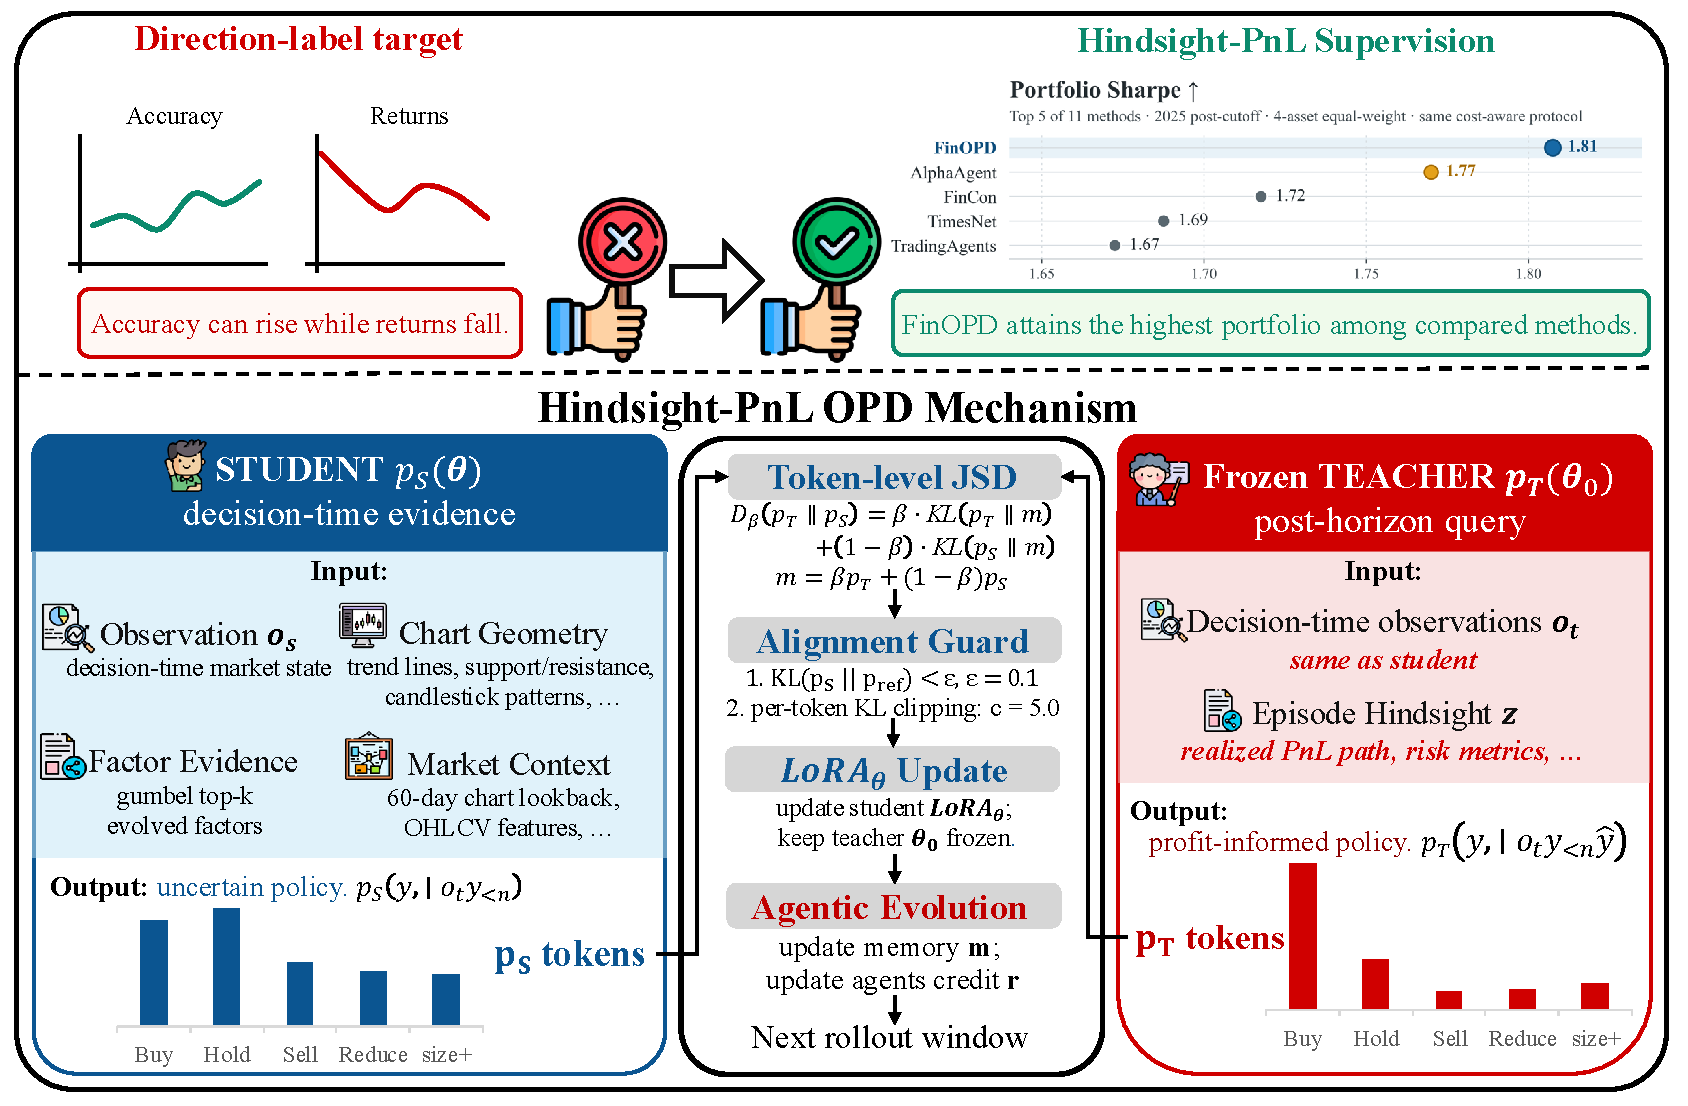
\includegraphics[width=0.95\columnwidth]{figures/FinOPD_mechanism.pdf}
\caption{On-policy distillation after horizon closure. The current student generates trajectories from decision-time evidence. A separate frozen teacher then receives only the estimated hindsight summary. Marginal agent credit weights token-level distillation, while a frozen round-start reference guards policy drift.}
% 中文翻译（图注）：结果窗口闭合后的在线策略蒸馏。当前学生只根据决策时证据生成轨迹；随后，独立冻结教师仅额外接收估计的事后摘要。智能体边际信用对 token 级蒸馏加权，冻结的 round-start reference 则约束策略漂移。
\Description{Diagram contrasting a deployable student conditioned only on current observations with a frozen teacher conditioned additionally on an estimated hindsight summary.}
\label{fig:opd}
\end{figure}

\paragraph{Post-horizon agent credit.}
Joint utility $U_t^H=u(\boldsymbol\xi_t^H)$ is shared. For coalition $S$, set $\widetilde m_t^j(S)=m_t^j$ if $j\in S$ and to role-typed null $m_\varnothing^j$ otherwise. Counterfactual replay on the same horizon gives
\begin{equation}
\label{eq:agent_credit}
\begin{aligned}
\mathbf w_t(S)&=D_{\eta}(
\{\widetilde m_t^j(S)\}_{j=1}^{A},F_t,E_t,\rho_t),\\
V_t(S)&=u\!\left(\operatorname{Evaluate}_H(
\mathbf w_t(S))\right),\\
\widehat\phi_{t,i}
&=\frac{1}{B}\sum_{b=1}^{B}
\left[V_t(P_i^{(b)}\cup\{i\})-V_t(P_i^{(b)})\right],\\
\omega_{t,i}&=
\frac{\exp(\widehat\phi_{t,i})}
{\sum_{j=1}^{A}\exp(\widehat\phi_{t,j})},
\qquad B=8.
\end{aligned}
\end{equation}
Here, $P_i^{(b)}$ precedes $i$ in sampled permutation $b$, so $\omega_{t,i}>0$ and $\sum_i\omega_{t,i}=1$. Post-horizon replay never changes the executed action; approximate credit only weights OPD.
% 中文翻译：联合成熟效用不能原样分配给所有智能体。对于智能体联盟 $S$，系统保留联盟内消息，并用角色类型匹配的空消息替换联盟外消息；冻结的受约束配置头随后在同一成熟窗口上重放反事实动作。通过 8 个随机排列估计每个智能体加入前后的边际贡献，再用 softmax 映射为严格为正且和为 1 的权重。联盟重放不会修改已经执行的原始动作；近似信用只是 OPD 的加权机制，不构成独立训练目标。

\paragraph{Token objective.}
For each assistant token, both discrepancies are full-vocabulary divergences:
\begin{equation}
\label{eq:opd_token}
\begin{aligned}
\bar p_{t,i,n}^{\theta}
&=\beta q_{t,i,n}^{\phi}
+(1-\beta)p_{t,i,n}^{\theta},\\
j_{t,i,n}^{\theta}
&=\beta D_{\mathrm{KL}}(
q_{t,i,n}^{\phi}\Vert\bar p_{t,i,n}^{\theta})
+(1-\beta)D_{\mathrm{KL}}(
p_{t,i,n}^{\theta}\Vert\bar p_{t,i,n}^{\theta}),\\
k_{t,i,n}^{\theta}
&=\min\!\left\{
D_{\mathrm{KL}}(q_{t,i,n}^{\phi}\Vert p_{t,i,n}^{\theta}),c
\right\},
\qquad
\ell_{t,i,n}^{\mathrm{OPD}}=j_{t,i,n}^{\theta}
+\lambda_{\mathrm{tok}}k_{t,i,n}^{\theta}.
\end{aligned}
\end{equation}
We use $\beta=0.5$, $c=5.0$, and $\lambda_{\mathrm{tok}}=0.1$. The KL is summed over the vocabulary before its non-negative scalar is clipped. Let $\mu_{t,i,n}$ mask assistant tokens and $\mathcal J_r=\{(t,i,n):b_t\in\mathcal B_r^H,1\leq i\leq A,1\leq n\leq|y_t^i|\}$ index matured responses. The normalized objective is
\begin{equation}
\label{eq:opd_loss}
\mathcal L_{\mathrm{OPD}}(\theta)=
\frac{\displaystyle
\sum_{(t,i,n)\in\mathcal J_r}\!
\mu_{t,i,n}\omega_{t,i}\ell_{t,i,n}^{\mathrm{OPD}}}
{\displaystyle
\sum_{(t,i,n)\in\mathcal J_r}\!
\mu_{t,i,n}\omega_{t,i}}.
\end{equation}
JSD provides bounded two-sided alignment, while clipped $q^\phi\Vert p^\theta$ retains directional teacher pressure; normalization removes dependence on response length and valid-token count. Outcomes enter only through the frozen teacher and post-horizon credit.
% 中文翻译：对于每个 assistant token 位置，广义 JSD 和教师--学生 KL 都在完整词表上定义。本文取 $\beta=0.5$、裁剪上限 $c=5.0$ 和暂定权重 $\lambda_{\mathrm{tok}}=0.1$。教师--学生 KL 会先对词表维度求和得到非负标量，再对该标量裁剪，而不是裁剪有正有负的单词项。OPD 目标只统计 assistant token，并按智能体信用加权后除以有效权重总和，因此不会随响应长度或有效 token 数量改变尺度。结果信息只通过冻结教师和结果成熟后的信用权重进入训练，学生输入仍严格保持时点安全。

\paragraph{Frozen-reference guard.}
The token cap controls a local teacher--student mismatch; a separate round-level guard controls cumulative drift of the language policy. For a candidate update $\theta'$ evaluated on the same prefixes, define
\begin{equation}
\label{eq:reference_kl}
\mathcal K_{\mathrm{ref}}(\theta';\theta_r)=
\frac{\displaystyle
\sum_{(t,i,n)\in\mathcal J_r}\!
\mu_{t,i,n}
D_{\mathrm{KL}}(p_{t,i,n}^{\theta'}\Vert
p_{t,i,n}^{\mathrm{ref}})}
{\displaystyle
\sum_{(t,i,n)\in\mathcal J_r}\mu_{t,i,n}}.
\end{equation}
We accept the candidate only if $\mathcal K_{\mathrm{ref}}(\theta';\theta_r)\leq\epsilon=0.1$; otherwise student and router revert to their round-start states. The guard directly constrains the student distribution; the router participates in the same transactional accept-or-revert step rather than being interpreted as KL-bounded. The teacher supplies the target, whereas the reference supplies the deployment anchor.
% 中文翻译：token 裁剪控制局部教师--学生失配，独立的轮级约束控制语言策略的累计漂移。候选学生在相同前缀上相对 round-start reference 计算平均 assistant-token KL；只有当该值不超过 $\epsilon=0.1$ 时才接受候选更新，否则学生与路由器一并回退到本轮开始状态。该 KL 直接约束学生分布；路由器只是参加同一个事务式“接受或回退”步骤，并不被表述为自身受到 KL 约束。教师提供事后信息辅助的训练目标，reference 提供部署锚点。

\subsection{Time-Safe Episodic Memory}
\label{sec:belief}

Parametric updates can average away rare, high-value situations, so we retain them as finalized episodes
\begin{equation}
\label{eq:episode_schema}
e_j=\bigl(\mathbf g_j,\mathbf r_j,F_j,\{m_j^i\},\mathbf w_j,
\boldsymbol\xi_j^H,t_j^{\mathrm{dec}},t_j^{\mathrm{end}},
t_j^{\mathrm{avail}}\bigr).
\end{equation}
Let $\mathcal U_r$ contain only utilities available by the close of round $r$. We admit episodes satisfying $t_j^{\mathrm{avail}}\geq t_j^{\mathrm{end}}>t_j^{\mathrm{dec}}$ and $U_j^H\geq Q_{0.8}(\mathcal U_r)$. At $C_{\max}=10{,}000$, we evict the lowest-utility entry.
% 中文翻译：参数更新能够吸收可复用行为，但可能把稀有高价值情形平均掉。因此，系统把图形嵌入、状态编码、因子、智能体消息、动作、成熟结果和三个时间戳保存为最终情节。$\mathcal U_r$ 只包含在第 $r$ 轮结束前已经可用的效用；只有结果窗口闭合、情节已经可用且效用达到该时点历史分布第 80 百分位时才允许写入。容量达到 10,000 后淘汰效用最低的条目。

Availability filtering precedes similarity search. With $\mathbf v_s=[\mathbf g_s;\mathbf r_s]$ for any time $s$, the eligible set and retrieved top-five episodes are
\begin{equation}
\label{eq:memory_score}
\begin{aligned}
\mathcal E_t&=\{e_j\in\mathcal M_r:t_j^{\mathrm{avail}}\leq t\},\\
E_t&=\underset{e_j\in\mathcal E_t}{\operatorname{arg\,top}\text{-}5}
\;\cos(\mathbf v_t,\mathbf v_j).
\end{aligned}
\end{equation}
The FAISS index~\cite{johnson2019billion} thus searches only knowable episodes and writes retrieved records to Gated Shared Memory as attributed priors, not labels.
% 中文翻译：相似度搜索之前必须先做可用时间过滤。系统把图形嵌入和市场状态编码拼接成检索向量，只在 $t_j^{\mathrm{avail}}\le t$ 的情节中按余弦相似度取前五项。因此，FAISS 索引不会检索查询时尚不可知的结果。取回的情节以带来源的先验写入 Gated Shared Memory，而不是作为监督标签，从而保持“召回”与“监督”的区别。

\subsection{Regime-Aware Selective Execution}
\label{sec:rasw}

We make the final aggregation within $D_\eta$ explicit. Let $s_{t,\ell}\in[-1,1]$ and $c_{t,\ell}\in[0,1]$ denote the calibrated direction and confidence of evidence channel $\ell$, including agent messages, routed-factor consensus, and retrieved priors. Regime-Adaptive Signal Weighting (RASW) uses non-negative regime weights $a_{\rho_t,\ell}$ and the Risk Controller multiplier $\chi_t\in[0,1]$ to compute
\begin{equation}
\label{eq:rasw}
\nu_t=\chi_t\,
\frac{\sum_{\ell}a_{\rho_t,\ell}c_{t,\ell}s_{t,\ell}}
{\sum_{\ell}a_{\rho_t,\ell}c_{t,\ell}}.
\end{equation}
We set $\nu_t=0$ when the denominator is zero. Edge-Gated Abstention then maps conviction to an action:
\begin{equation}
\label{eq:selective_execution}
\delta_t=
\begin{cases}
\textsc{Buy}, & \nu_t>\kappa^+(\rho_t),\\
\textsc{Sell}, & \nu_t<\kappa^-(\rho_t),\\
\textsc{Hold}, & \text{otherwise}.
\end{cases}
\end{equation}
For trending or volatile regimes, $(\kappa^+,\kappa^-)=(0.15,-0.25)$; otherwise they are $(0.60,-0.70)$. Position sizing maps $\delta_t$ to $\mathbf w_t\in\mathcal W_t$ while applying the Risk Controller veto, transaction costs, a volatility-conditioned holding horizon, and trend-break exits. We treat RASW and EGA as supporting components inside Regime-Aware Selective Execution, not additional agents.
% 中文翻译：这里展开的是 $D_\eta$ 内部的最终聚合步骤。每个证据通道都给出 $[-1,1]$ 区间的校准方向和 $[0,1]$ 区间的置信度，通道包括智能体消息、路由因子共识和检索先验。RASW 使用非负的状态条件权重，并乘以 Risk Controller 给出的风险缩放系数，形成统一置信分数。EGA 在趋势或高波动状态采用 $(0.15,-0.25)$ 的买卖阈值，在其他状态采用更保守的 $(0.60,-0.70)$；未越过阈值时保持不交易。仓位步骤把离散动作 $\delta_t$ 映射为 $\mathbf w_t\in\mathcal W_t$，同时应用风险否决、交易成本、波动率条件持有期和趋势断裂退出。RASW 与 EGA 是 Regime-Aware Selective Execution 内部的辅助组件，不是额外智能体。

Algorithm~\ref{alg:finopd} separates point-in-time rollout from post-horizon annotation, optimization, and memory admission.
% 中文翻译：算法 1 把一轮进化严格划分为两个互不混合的阶段。阶段 I 中的全部对象都必须在决策时可得；成熟结果、估计事后摘要、智能体信用、参数更新和记忆写入只允许出现在阶段 II。

\begin{algorithm}[t]
\caption{\textsc{FinOPD}: One Self-Evolution Round}
\label{alg:finopd}
\footnotesize
\begin{algorithmic}[1]
\REQUIRE $\pi_{\theta_r},q_{\phi},R_{\psi_r},D_{\eta},\mathcal F^\star,\mathcal M_r,H,\mathcal T_r,t_r^{\mathrm{close}}$
\STATE $\pi^{\mathrm{ref}}\gets\operatorname{Freeze}(\pi_{\theta_r})$;
$\mathcal B_r\gets\varnothing$
\STATE \textsc{Phase I: Point-in-time rollout}
\FOR{$t\in\mathcal T_r$}
\STATE $(\mathbf g_t,\rho_t)\gets\operatorname{Encode}(o_t)$
\STATE $E_t\gets\operatorname{Retrieve}(\mathcal M_r,t,\mathbf g_t,\rho_t)$
\STATE $F_t\gets\operatorname{Route}(R_{\psi_r},\mathcal F^\star,\mathbf g_t,\rho_t)$
\STATE $(\{y_t^i,m_t^i\}_{i=1}^{A},\mathcal G_t)
\gets\operatorname{Agents}(\pi_{\theta_r},o_t,F_t,E_t)$
\STATE $\mathbf w_t\gets D_{\eta}(\mathcal G_t,F_t,E_t,\rho_t)$;
$\operatorname{Execute}(\mathbf w_t)$
\STATE $\mathcal B_r\gets\mathcal B_r\cup
\{(t,o_t,F_t,E_t,\mathcal G_t,\{y_t^i\},\mathbf w_t)\}$
\ENDFOR
\STATE \textsc{Phase II: Post-horizon update}
\STATE $\mathcal B_r^H\gets\{b_t\in\mathcal B_r:t+H\leq t_r^{\mathrm{close}}\}$
\FOR{$b_t\in\mathcal B_r^H$}
\STATE $\boldsymbol\xi_t^H\gets\operatorname{Evaluate}_H(\mathbf w_t)$;
$\widehat{\mathbf h}_t^H\gets\operatorname{Summarize}(\boldsymbol\xi_t^H)$
\STATE $\{q_{t,i,n}^{\phi}\}\gets q_{\phi}(b_t,\widehat{\mathbf h}_t^H)$;
$\boldsymbol\omega_t\gets\operatorname{Credit}(b_t,\boldsymbol\xi_t^H)$
\ENDFOR
\STATE $\theta'\gets\operatorname{Update}(\theta_r,\mathcal L_{\mathrm{OPD}})$;
$\psi'\gets\operatorname{Update}(\psi_r,\mathcal L_{\mathrm{route}})$
\IF{$\mathcal K_{\mathrm{ref}}(\theta';\theta_r)\leq\epsilon$}
\STATE $(\theta_{r+1},\psi_{r+1})\gets(\theta',\psi')$
\ELSE
\STATE $(\theta_{r+1},\psi_{r+1})\gets(\theta_r,\psi_r)$
\ENDIF
\STATE $\mathcal C_r\gets\{\operatorname{Episode}(b_t):
b_t\in\mathcal B_r^H,U_t^H\geq Q_{0.8}(\mathcal U_r)\}$
\STATE $\mathcal M_{r+1}\gets\operatorname{Cap}(\mathcal M_r\cup\mathcal C_r,C_{\max})$
\RETURN $\theta_{r+1},\psi_{r+1},\mathcal M_{r+1}$
\end{algorithmic}
\end{algorithm}
% 中文翻译（算法）：阶段 I 冻结 round-start reference，并在每个决策时点依次执行编码、时间安全检索、因子路由、五智能体消息生成、组合决策与真实执行，同时保存完整的 on-policy 记录。阶段 II 只处理已经跨过结果窗口的记录：计算成熟结果与估计事后摘要，调用冻结教师，重放联盟以获得信用权重，分别更新学生和路由器；若候选学生违反 reference KL 预算，则学生与路由器共同回退。最后仅将达到 80 分位效用门槛的成熟情节写入有容量约束的记忆，冻结因子库始终不变。
\endgroup
